\section{Studio della risoluzione del rivelatore}

Vogliamo caratterizzare la risoluzione del rivelatore:
\begin{equation} 
R = \frac{\Delta E}{E}
\end{equation}
dove $ \Delta E $ è la larghezza del picco a energie $ E $ misurato dal rivelatore.

In particolare, abbiamo calcolato $ \Delta E $ usando la formula:
\begin{equation}
\Delta E = b \qty(C_\text{dx} - C_\text{sx}) + c \qty(C_\text{dx}^{2} - C_\text{sx}^{2})
\end{equation}
dove $ a $ e $ b $ sono i parametri di calibrazione calcolati in \cref{eq:calibration}, mentre i canali $ C $ destro e sinistro corrispondono ai punti a metà altezza di ogni picco:
\begin{equation}
C_\text{sx} = C_\text{peak} - \frac{\text{FWHM}_\text{peak}}{2} \qquad C_\text{dx} = C_\text{peak} + \frac{\text{FWHM}_\text{peak}}{2}.
\end{equation}

Per propagare gli errori su posizioni e larghezze dei picchi abbiamo considerato le stime fatte in \cref{sec:errcentr}, mentre abbiamo trascurato la covarianza tra il parametro $ b $ e il parametro $ c $.\footnote{Esplicitando la formula del calcolo di $ \Delta E $ (senza calcolare $ E_\text{sx} \pm \delta E_\text{sx} $ e $ E_\text{dx} \pm \delta E_\text{dx} $, per poi prenderne la differenza) elimina, già, il contributo dell'errore su $ a $ dalla stima.} 

Il modello teorico che abbiamo usato per descrivere l'andamento della risoluzione è:
\begin{equation} \label{eq:resolution}
R = \frac{k}{\sqrt{E}} + c
\end{equation}
dove $ k $ rappresenta \help{??? è rumore statistico}, mentre $ c $ un contributo di fondo del sistema.

Nello specifico, per effettuare la regressione (in \cref{fig:resolution}) abbiamo utilizzato solo i dati relativi ai fotopicchi di \ce{^60Co}, \ce{^137Cs}, e \ce{^22Na}, come in \cref{tab:resolution}
Troviamo che la regressione converge in maniera accettabile per i parametri:
\begin{equation}
k = (6.5 \pm 1.2) \cdot 10^{-2} \unit{MeV^{1/2}} \qquad c = (0.000 \pm 0.012 )
\end{equation}
e usando questi valori per calcolare la risoluzione del rilevatore a $ 1 \unit{MeV} $ troviamo $ R(1 \unit{MeV}) = 6.5 \% $, che è un valore tipico per i rivelatori \ce{NaI(Tl)}.
Osserviamo anche che il parametro $ c $ è compatibile con $ 0 $: il contributo di fondo del sistema non è rilevante, almeno nel range di energie che abbiamo studiato.

\begin{figure}
\centering
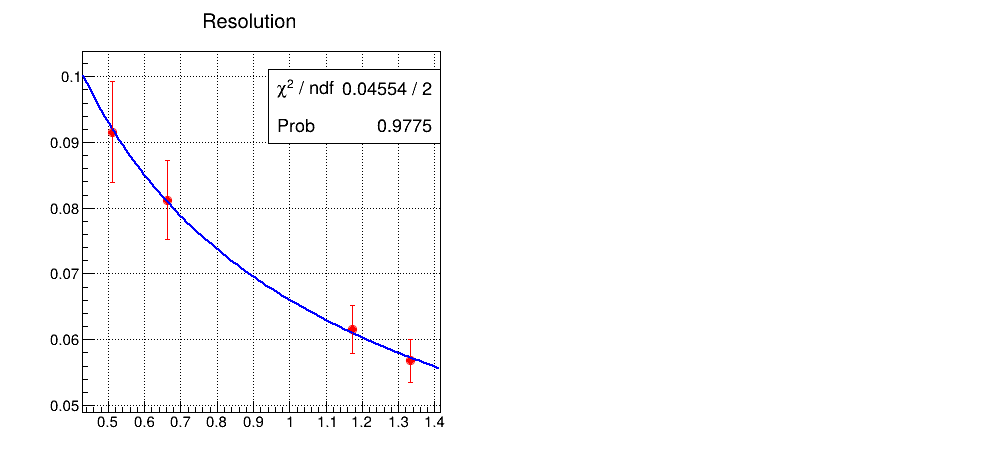
\includegraphics[scale=0.5]{images/energeticResolution.png}
\caption{Regressione con il modello (\ref{eq:resolution}) ai dati in \cref{tab:resolution} per caratterizzare l'andamento della risoluzione $ R = \Delta E / E $ del rivelatore contro l'energia $ E $.}
\label{fig:resolution}
\end{figure}

\begin{table}
    \centering
    \begin{tabular}{c|cc|cc|cc|cc}
        sorgente & $ E [\unit{MeV}] $ & $\delta E [\unit{MeV}] $ & centroide & $ \delta $ centroide & FWHM & $ \delta $ FWHM & $ R \qty(\frac{\Delta E}{E}) $ & $ \delta R $ \\
        \hline
        \ce{^22Na} & 0.5110 & 0.0010 & 307.2 & 1.5 & 27.1 & 0.7 &0.092 & 0.008 \\
        \ce{^60Co} - 1 & 1.1732 & 0.0010 & 685.0 & 1.5 & 41.2 & 0.7 & 0.062 & 0.004 \\
        \ce{^60Co} - 2 & 1.3325 & 0.0010 & 780.5 & 1.5 & 43.0 & 0.7 & 0.057 & 0.003 \\
        \ce{^137Cs} & 0.66166 & 0.00010 & 395.4 & 1.5 & 31.0 & 0.7 &0.081 & 0.006 \\
    \end{tabular}
    \caption{Dati relativi al fit in \cref{fig:resolution}: abbiamo usato i valori di energia teorici $ E $, e li abbiamo confrontati con la FWHM in energia per ogni picco calcolata a partire dalla FWHM in canali (stimata dal software). Abbiamo usato come errori sulle stime dei centroidi e della FWHM le deviazioni standard delle misure ripetute di \ce{^60Co}.}
    \label{tab:resolution}
\end{table}

\section{Misura dell'attività di una sorgente}

Abbiamo acquisito gli spettri di due sorgenti di \ce{^137Cs} (etichettate FS65 e FS66) per determinarne l'attività, sia con un metodo relativo che con uno assoluto.

\begin{figure}[]
    \centering

    \subcaptionbox{Sorgente FS65 \label{fig:fs65}}
    {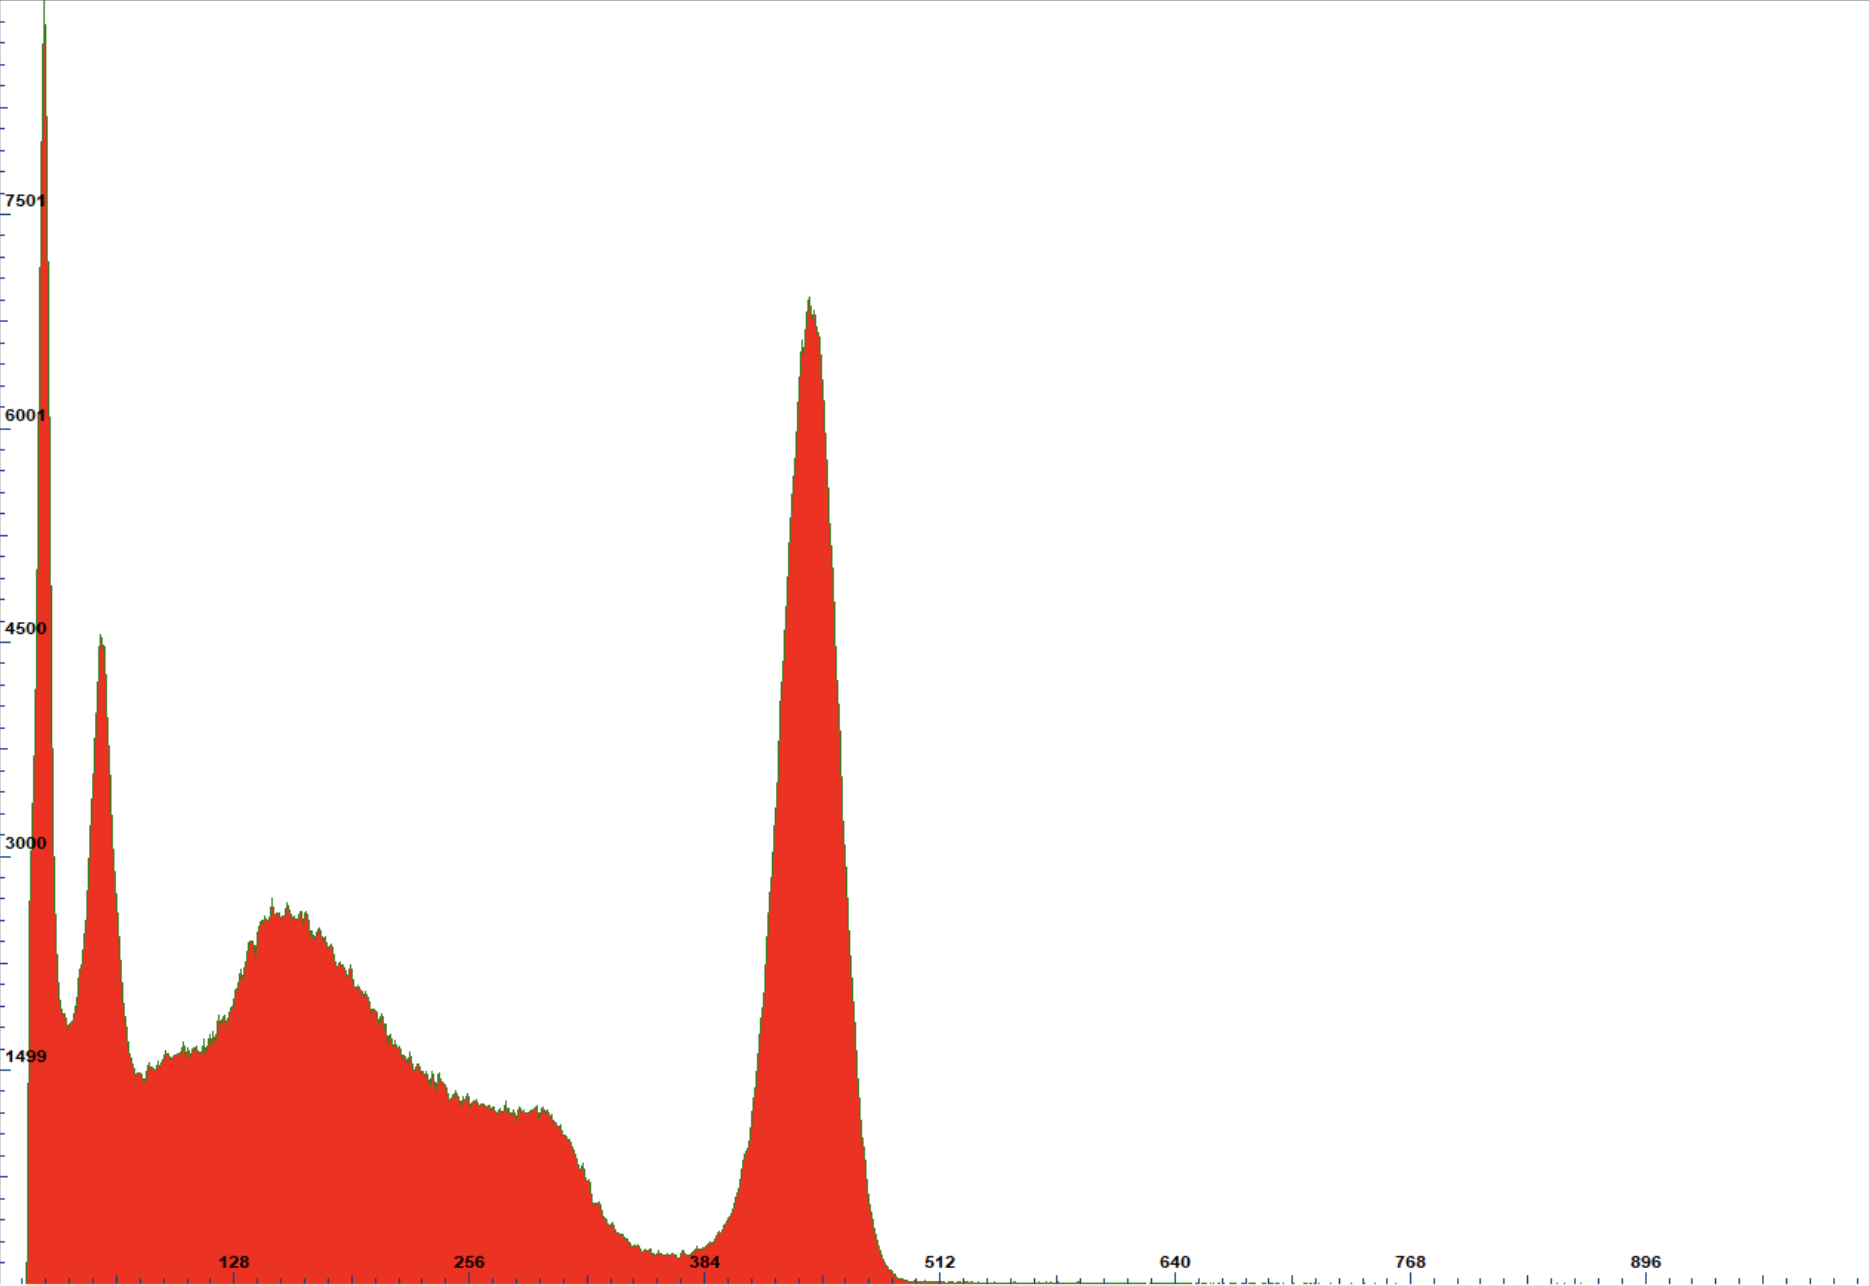
\includegraphics[width=0.45\textwidth]{images/fs65.png}}
    \hfill
    \subcaptionbox{Sorgente FS66 \label{fig:fs66}}
        {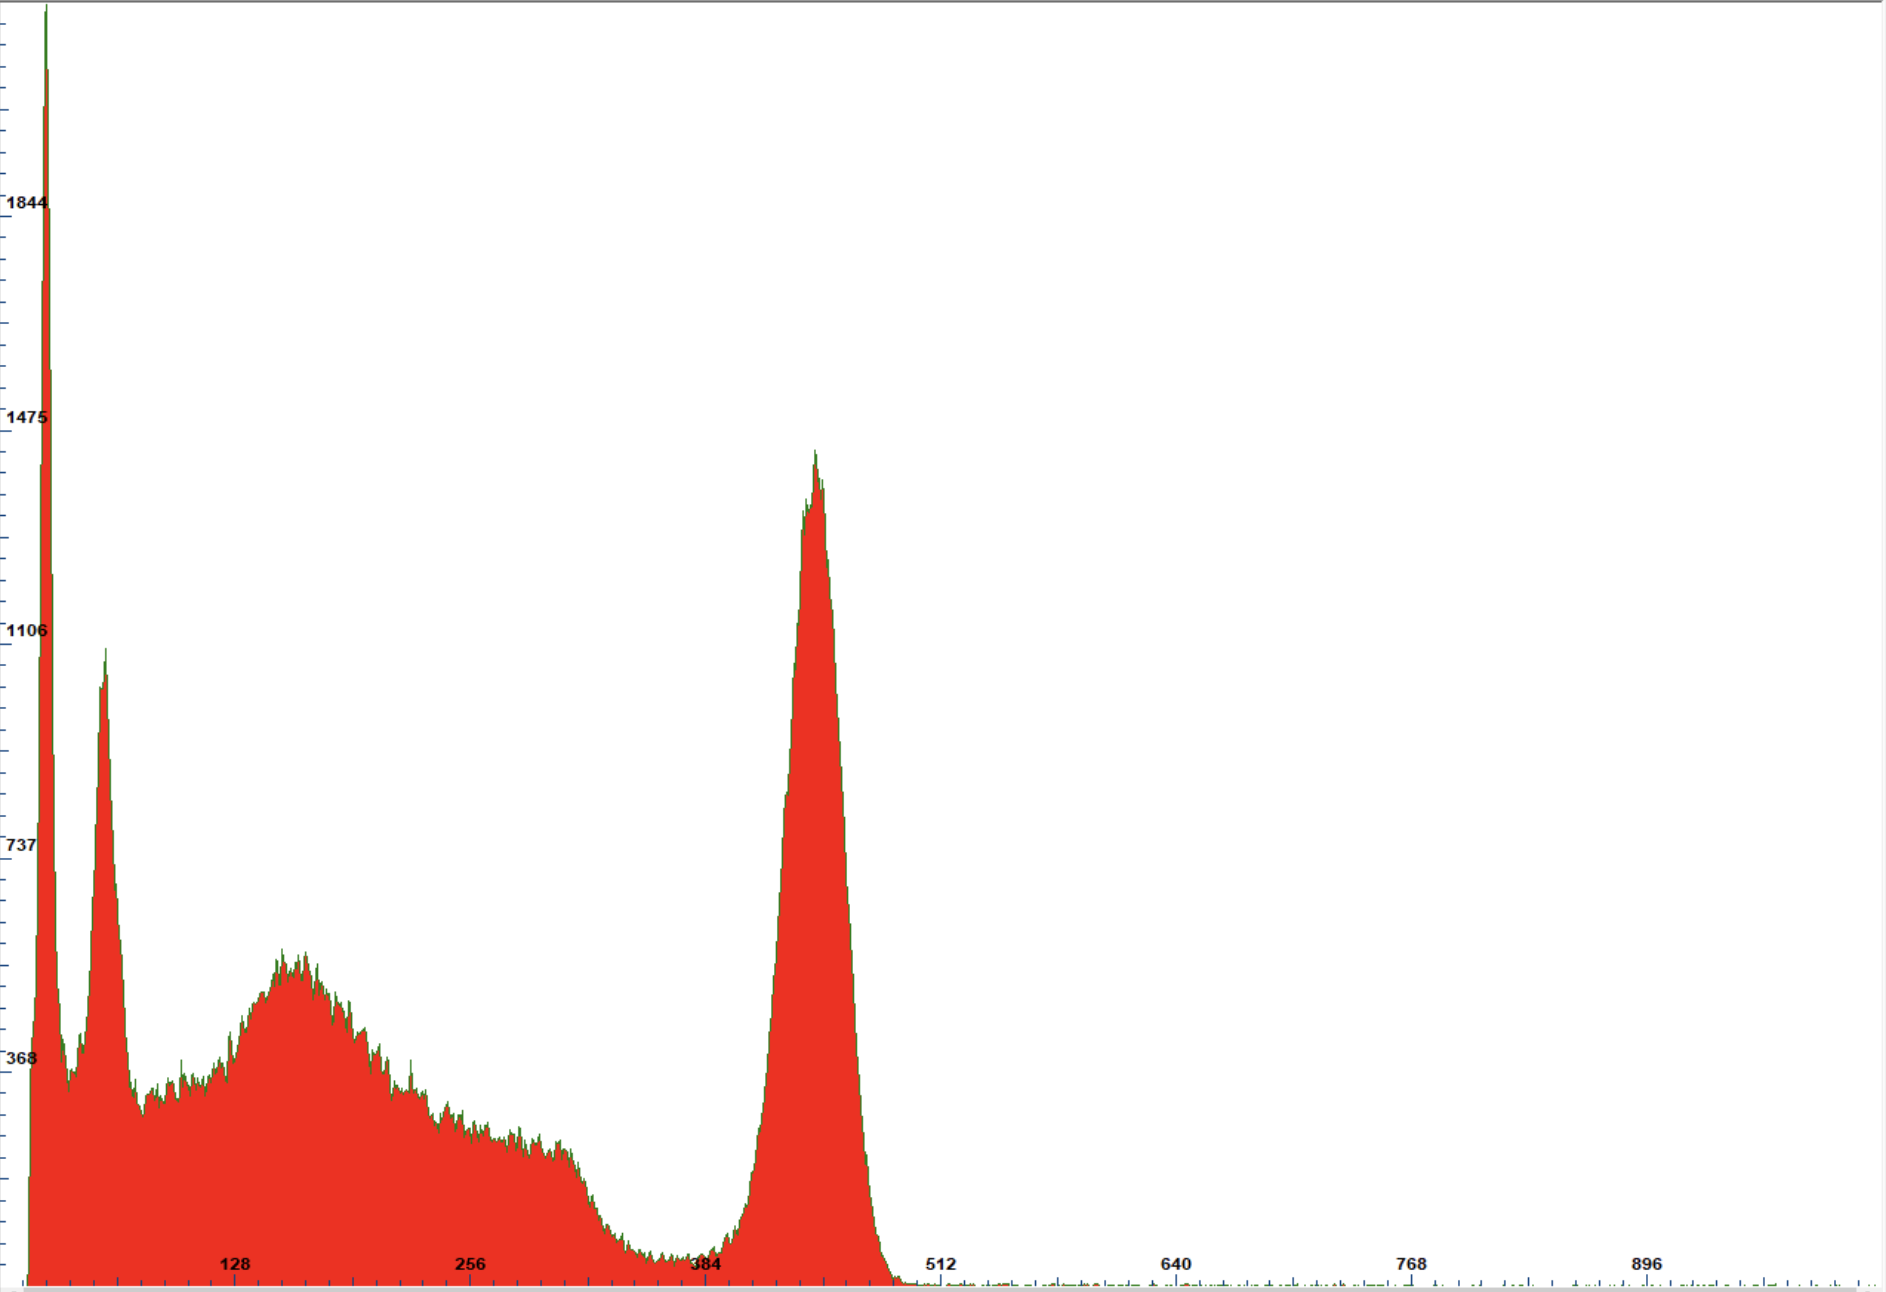
\includegraphics[width=0.45\textwidth]{images/fs66.png}}

        \caption{Spettri delle sorgenti di \ce{^137Cs} FS65 e FS66 di cui abbiamo determinato le attività. Anche se i tempi di misura $ t_\text{live} $ sono pressoché identici l'altezza del picco della sorgente FS65 è chiaramente maggiore di quella della sorgente FS66 (le scale degli assi verticali sono diverse nei due grafici).}
    \label{fig:activityspectra}
\end{figure}

Le attività nominali delle sorgenti sono note al 07/11/2024:
\begin{equation}
A_\text{FS65} = (193 \pm 10)\unit{kBq} \qquad  A_\text{FS66} = (37.4 \pm 1.9) \unit{kBq}
\end{equation}
e considerando il tempo di dimezzamento del \ce{^137Cs}:
\begin{equation}
t_{1/2} = (30.150 \pm 0.010) \unit{y}
\end{equation}
abbiamo utilizzato la legge di decadimento esponenziale per calcolare le attività tabulate al giorno dell'esperienza (14/04/2026, cioè $ \Delta t = (1.432 \pm 0.003) \unit{y} $):
\begin{equation} \label{eq:expdec}
A = A_0e^{-\lambda\Delta t}
\end{equation}
ottenendo:
\begin{equation}\label{eq:csactivities}	
A_\text{FS65,today} = (187 \pm 9) \unit{kBq} \qquad A_\text{FS66,today} = (36.2 \pm 1.8) \unit{kBq}.
\end{equation}

In particolare, per applicare entrambi i metodi abbiamo misurato i rate dei picchi fotoelettrici delle due sorgenti stimandoli usando:
\begin{equation}
R = \frac{A_n}{t_\text{live}}
\end{equation}
come riportato in \cref{tab:csrates}, dove $ A_n $ è il numero di conteggi netti (con errore calcolato a partire dai conteggi lordi $ A_g $ come illustrato in \cref{sec:errnetcounts}) e $ t_\text{live} $ il tempo di misura a cui è stato sottratto il tempo morto. 

\begin{table}
	\centering
	\begin{tabular}{c|cccccc}
		sorgente & $A_n$ & $A_g$ & $t_\text{live} \, [\unit{s}]$ & $\delta t_\text{live} \, [\unit{s}]$ & $R \, [\unit{s^{-1}}]$ & $\delta R \, [\unit{s^{-1}}]$ \\
		\hline
		FS65 & 257764 & 273300  & 349.150 & 0.010 & 738.3 & 1.5 \\ 
		FS66 & 51439 & 55415 & 354.170 & 0.010  & 145.2 & 0.7 
	\end{tabular}
	\caption{Dati relativi al conteggio dei rate del picco fotoelettrico delle due sorgenti di \ce{^137Cs}: l'area netta del picco $A_n$ determinata dal software rimuovendo il background all'area lorda $A_g$ (espresse entrambe in numero di conteggi), il tempo di misura $t_\text{live}$ e i rate con il loro errore.}
	\label{tab:csrates}
\end{table}

\subsection{Attività della sorgente con il metodo relativo}

Il metodo relativo ci permette di ricavare l'attività di una sorgente incognita (FS66) conoscendo quella di una sorgente nota (FS65) sfruttando la proporzionalità diretta tra attività e rate di conteggi $ A \propto R $:
\begin{equation}
A_x = A_s\frac{R_x}{R_s}.
\end{equation}	

Quindi, usando i dati in \cref{tab:csrates} abbiamo calcolato l'attività della sorgente FS66:
\begin{equation}
A_\text{FS66,rel} = (36.8 \pm 1.9) \unit{kBq} 
\end{equation}
e confrontandola con quella teorica in \cref{eq:csactivities} con un test Z abbiamo trovato che è compatibile ($ Z = 0.207 $ e $ p = 0.836 $) al 5\%.

\subsection{Attività delle sorgenti con il metodo assoluto}

Per utilizzare il metodo assoluto sfruttiamo la relazione seguente:
\begin{equation}\label{eq:absactivity}
	A = \frac{R}{\epsilon G f_g}
\end{equation}
dove $R$ sono i rate, $\epsilon$ è l'efficienza del rivelatore, $G$ è l'accettanza mentre $f_g$ è la frazione di decadimento.
In particolare abbiamo calcolato $G$ con la seguente relazione:
\begin{equation} \label{eq:acc}
G = \frac{1}{2}\qty[1-\cos(\arctan(\frac{a}{d}))].
\end{equation}

Nello specifico nel nostro setup:\footnote{Il valore dell'efficienza $\epsilon$ dipende sia dall'energia dei $\gamma$ incidenti, sia da fattori geometrici: questa stima è valida per il picco di emissione del \ce{^137Cs} alla distanza $ d = 9.3 \unit{cm} $.}
\begin{equation}
\epsilon = (0.25 \pm 0.01) \quad f_g = 0.851 \quad a = (2.5 \pm 0.1) \unit{cm} \quad d = (9.3 \pm 0.1) \unit{cm}
\end{equation}
e quindi abbiamo valutato l'accettanza come $ G = (0.0177 \pm 0.0013)$ (usando l'\cref{eq:acc}).

Usando l'equazione in \cref{eq:absactivity} con i rates in \cref{tab:csrates} abbiamo ricavato:
\begin{equation}
A_\text{FS65,abs} = (196 \pm 17) \unit{kBq} \qquad A_\text{FS66,abs} = (38\pm3) \unit{kBq}
\end{equation}
Valori che se confrontati con quelli in \cref{eq:csactivities} con un test Z risultano essere compatibili ($Z_{65} = 0.727$, $ p_{65} = 0.467$ e $Z_{66} = 0.956$, $ p_{66} = 0.399$) al 5\%.  
